% HOT overview figure, redrawn in the thesis font. Compile with pdflatex.
\documentclass[border=0pt]{standalone}
\usepackage[T1]{fontenc}
\IfFileExists{newpxtext.sty}{\usepackage{newpxtext,newpxmath}}{\usepackage{pxfonts}} % thesis font
\usepackage{tikz}
\definecolor{hotnavy}{HTML}{2B3A67}  \definecolor{hotnavyfill}{HTML}{E3E7F2}
\definecolor{hotteal}{HTML}{1F8A80}  \definecolor{hottealfill}{HTML}{DDF1EE}
\definecolor{hotamber}{HTML}{C98A1B} \definecolor{hotamberfill}{HTML}{FBEFD6}
\definecolor{hotambertext}{HTML}{9A6A10}
\definecolor{ink}{HTML}{1C2233}      \definecolor{muted}{HTML}{5B6170}
\begin{document}\frenchspacing
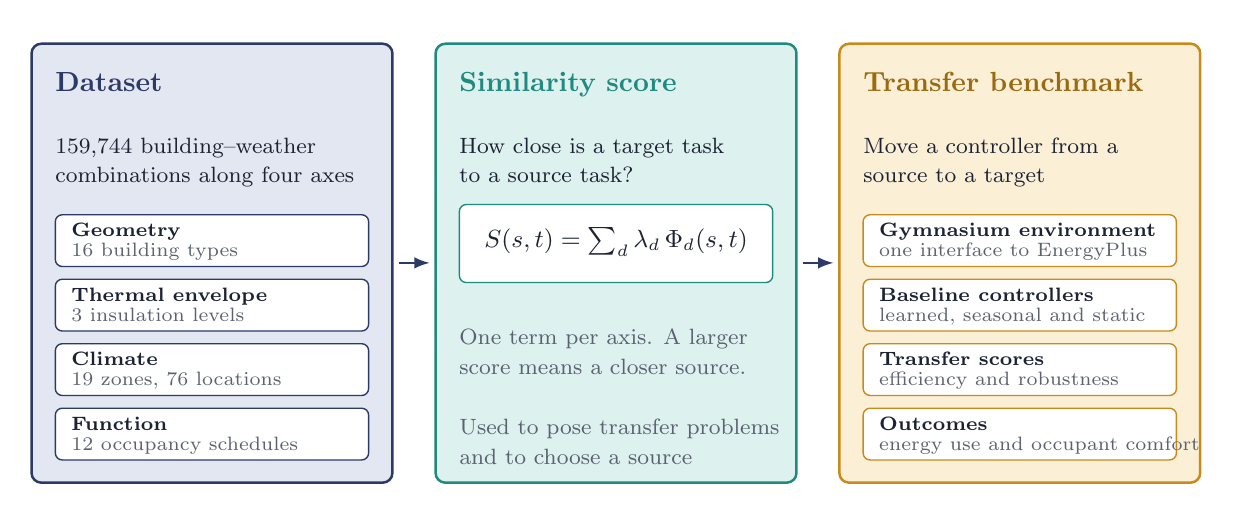
\begin{tikzpicture}[x=1pt,y=-1pt,
  every node/.style={inner sep=0pt,outer sep=0pt,anchor=base west,text=ink},
  panel/.style={rounded corners=3.5pt,line width=0.9pt},
  item/.style={rounded corners=2.5pt,line width=0.5pt,fill=white},
  head/.style={font=\fontsize{10}{12}\selectfont\bfseries},
  body/.style={font=\fontsize{7.8}{10}\selectfont},
  name/.style={font=\fontsize{7.2}{9}\selectfont\bfseries},
  sub/.style={font=\fontsize{6.6}{8}\selectfont,text=muted}]
\useasboundingbox (0,0) rectangle (425.2,170.1);

% item box: #1 x-offset of panel, #2 top y, #3 border colour, #4 name, #5 description
\newcommand{\hotitem}[5]{%
  \draw[item,draw=#3] (#1+8.6,#2) rectangle (#1+121.8,#2+18.7);
  \node[name] at (#1+14.4,#2+7.9) {#4};
  \node[sub]  at (#1+14.4,#2+15.2) {#5};}

% ---- Dataset ----
\draw[panel,draw=hotnavy,fill=hotnavyfill] (1.4,5.8) rectangle (131.8,164.4);
\node[head,text=hotnavy] at (10,23.2) {Dataset};
\node[body] at (10,45.6) {159,744 building--weather};
\node[body] at (10,56.0) {combinations along four axes};
\hotitem{1.4}{67.6}{hotnavy}{Geometry}{16 building types}
\hotitem{1.4}{90.9}{hotnavy}{Thermal envelope}{3 insulation levels}
\hotitem{1.4}{114.2}{hotnavy}{Climate}{19 zones, 76 locations}
\hotitem{1.4}{137.5}{hotnavy}{Function}{12 occupancy schedules}

% ---- Similarity score ----
\draw[panel,draw=hotteal,fill=hottealfill] (147.4,5.8) rectangle (277.8,164.4);
\node[head,text=hotteal] at (156,23.2) {Similarity score};
\node[body] at (156,45.6) {How close is a target task};
\node[body] at (156,56.0) {to a source task?};
\draw[item,draw=hotteal] (156,63.9) rectangle (269.2,92.1);
\node[anchor=center,font=\fontsize{9}{11}\selectfont] at (212.6,77.6)
  {$S(s,t)=\sum_{d}\lambda_d\,\Phi_d(s,t)$};
\node[body,text=muted] at (156,114.6) {One term per axis. A larger};
\node[body,text=muted] at (156,125.2) {score means a closer source.};
\node[body,text=muted] at (156,147.1) {Used to pose transfer problems};
\node[body,text=muted] at (156,157.7) {and to choose a source};

% ---- Transfer benchmark ----
\draw[panel,draw=hotamber,fill=hotamberfill] (293.3,5.8) rectangle (423.7,164.4);
\node[head,text=hotambertext] at (302,23.2) {Transfer benchmark};
\node[body] at (302,45.6) {Move a controller from a};
\node[body] at (302,56.0) {source to a target};
\hotitem{293.3}{67.6}{hotamber}{Gymnasium environment}{one interface to EnergyPlus}
\hotitem{293.3}{90.9}{hotamber}{Baseline controllers}{learned, seasonal and static}
\hotitem{293.3}{114.2}{hotamber}{Transfer scores}{efficiency and robustness}
\hotitem{293.3}{137.5}{hotamber}{Outcomes}{energy use and occupant comfort}

% ---- arrows ----
\foreach \x in {134.2,280.1}
  \draw[hotnavy,line width=0.9pt,-{latex}] (\x,85) -- (\x+11,85);
\end{tikzpicture}
\end{document}
